\chapter{Il progetto e il suo sviluppo}\label{chapter:formattazione}
%
\section{Database}\label{sec:cap_sec_subsec}
Una parte sostanziale del nostro impegno aziendale per portare a compimento il 
progetto si è concentrata in modo dettagliato sulla creazione del database, ritenuto 
elemento cruciale per assicurare il pieno funzionamento della piattaforma.
\\ \\
La creazione del database è stata articolata in diverse fasi chiave:
\begin{itemize}
	\item Progettazione della struttura del database, un processo attentamente studiato.
	\item Scrittura del database in linguaggio SQL, una tappa essenziale.
	\item Implementazione delle interrogazioni al database nella sezione di backend, facendo uso della libreria Dapper.
\end{itemize}
\textit{Nota}: il database è stato creato e gestito unicamente in locale per questioni di semplicità e per
l'esecuzione di test sulla correttezza della struttura e dell'implementazione del database stesso.
%
%
\subsection{Progettazione}
La fase di progettazione~\ref{fig:one} del database ha occupato un ruolo fondamentale nel corso di 
questo processo, coinvolgendo un'analisi costante e una riflessione profonda. Il nostro 
obiettivo principale era plasmare un database estremamente completo, in grado di 
soddisfare appieno le esigenze della piattaforma di e-learning. In aggiunta, ci siamo 
concentrati su:
\begin{itemize}
	\item Migliorare la leggibilità del database;
	\item Rendere più agevole la manutenzione;
	\item Fornire ampie possibilità di estensione del sistema.
\end{itemize}
\begin{figure}[ht]
	\centering
	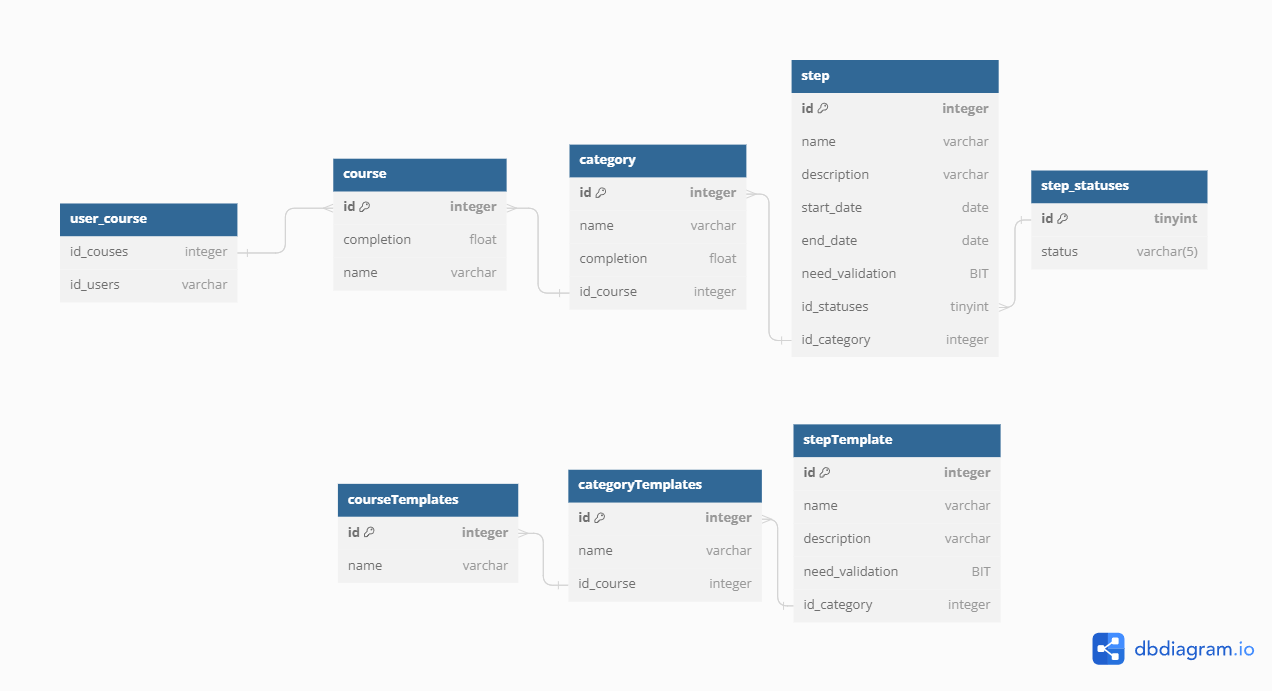
\includegraphics[width=1\textwidth]{img/progettazione_database.png}
	\caption{progettazione del database}
	\label{fig:one}
\end{figure}
\textit{Nota}: la progettazione mostrata non tiene traccia delle tabelle utente, perchè vengono 
gestite automaticamente dal progetto .NET grazie al servizio di autenticazione già 
incluso (libreria \inlinecode{Microsoft.EntityFrameworkCore.Migrations;}). 
%
\subsection{Scrittura nel linguaggio SQL}
Il risultato finale di questa fase è il seguente (non sono riportate le tabelle generate dal 
servizio di Autenticazione, perchè gestite automaticamente dalla libreria a disposizione):
\begin{lstlisting}[language=SQL, caption=traduzione della progettazione del database nel linguaggio SQL]
CREATE TABLE [dbo].[Course] ( 
    [Id]         INT            IDENTITY (1, 1) NOT NULL, 
    [Name]       NVARCHAR (255) NOT NULL, 
    [Completion] REAL           DEFAULT ((0)) NULL, 
    [StartDate]  DATETIME2 (7)  NULL, 
    [EndDate]    DATETIME2 (7)  NULL, 
    CONSTRAINT [PK_Course] PRIMARY KEY CLUSTERED ([Id] ASC) 
); 

CREATE TABLE [dbo].[Category] ( 
    [Id]         INT            IDENTITY (1, 1) NOT NULL, 
    [Name]       NVARCHAR (255) NOT NULL, 
    [Completion] REAL           DEFAULT ((0)) NULL, 
    [IdCourse]   INT            NOT NULL, 
    CONSTRAINT [PK_Category] PRIMARY KEY CLUSTERED ([Id] ASC), 
    CONSTRAINT [FK_Category_Course_IdCourse]
	FOREIGN KEY ([IdCourse]) REFERENCES [dbo].[Course] ([Id]) 
	ON DELETE CASCADE 
   ); 
   GO 
   CREATE NONCLUSTERED INDEX [IX_Category_IdCourse] 
	   ON [dbo].[Category]([IdCourse] ASC); 	

-- 3 stati: 
	-- 1. done 
	-- 2. todo 
	-- 3. check 
CREATE TABLE [dbo].[StepStatus] ( 
	[Id]     INT            IDENTITY (1, 1) NOT NULL, 
	[Status] NVARCHAR (10) NOT NULL, 
	CONSTRAINT [PK_StepStatus] PRIMARY KEY CLUSTERED ([Id] ASC) 
); 
	
CREATE TABLE [dbo].[Step] ( 
	[Id]             INT            IDENTITY (1, 1) NOT NULL, 
	[Name]           NVARCHAR (255) NOT NULL, 
	[Description]    NVARCHAR (MAX) NULL, 
	[StartDate]      DATETIME2 (7)  NULL, 
	[EndDate]        DATETIME2 (7)  NULL, 
	[Lock]           BIT            DEFAULT ((1)) NULL, 
	[NeedValidation] BIT            DEFAULT ((0)) NULL, 
	[IdStatus]       INT            DEFAULT ((1)) NULL, 
	[IdCategory]     INT            NOT NULL, 
	CONSTRAINT [PK_Step] PRIMARY KEY CLUSTERED ([Id] ASC), 
	CONSTRAINT [FK_Step_StepStatus_IdStatus]  
FOREIGN KEY ([IdStatus]) REFERENCES [dbo].[StepStatus] ([Id]) 
ON DELETE CASCADE, 
	CONSTRAINT [FK_Step_Category_IdCategory]  
FOREIGN KEY ([IdCategory]) REFERENCES [dbo].[Category] ([Id]) 
ON DELETE CASCADE 
); 
GO 
CREATE NONCLUSTERED INDEX [IX_Step_IdCategory] 
	ON [dbo].[Step]([IdCategory] ASC); 
GO 
CREATE NONCLUSTERED INDEX [IX_Step_IdStatus] 
	ON [dbo].[Step]([IdStatus] ASC); 

CREATE TABLE [dbo].[UserCourse] ( 
	[UserId]   NVARCHAR (450) NOT NULL, 
	[CourseId] INT            NOT NULL, 
	CONSTRAINT [FK_UserCourse_Course_CourseModel]  
FOREIGN KEY ([CourseId]) REFERENCES [dbo].[Course] ([Id]) 
ON DELETE CASCADE, 
	CONSTRAINT [FK_UserCourse_AspNetUsers_UserId]  
FOREIGN KEY ([UserId]) REFERENCES [dbo].[AspNetUsers] ([Id]) 
ON DELETE CASCADE 
); 
GO 
CREATE NONCLUSTERED INDEX [IX_UserCourse_CourseModel] 
    ON [dbo].[UserCourse]([CourseId] ASC); 
GO 
CREATE NONCLUSTERED INDEX [IX_UserCourse_UserId] 
    ON [dbo].[UserCourse]([UserId] ASC); 
 
CREATE TABLE [dbo].[CourseTemplate] ( 
    [Id]             INT            IDENTITY (1, 1) NOT NULL, 
    [Name]           NVARCHAR (255) NOT NULL, 
    [Creator]        NVARCHAR (255) NOT NULL, 
    [CreationDate]   DATETIME2 (7)  NULL, 
    [LastUpdateDate] DATETIME2 (7)  NULL, 
    CONSTRAINT [PK_CourseTemplate] PRIMARY KEY CLUSTERED ([Id] ASC) 
); 
 
CREATE TABLE [dbo].[CategoryTemplate] ( 
    [Id]                INT         IDENTITY (1, 1) NOT NULL, 
    [name]              NCHAR (255) NOT NULL, 
    IDCourseTemplate INT         NOT NULL, 
    PRIMARY KEY CLUSTERED ([Id] ASC), 
    FOREIGN KEY (IDCourseTemplate)  
 REFERENCES [dbo].[CourseTemplate] ([Id]) 
 ON DELETE CASCADE 
); 
 
CREATE TABLE [dbo].[StepTemplate] ( 
    [Id]                 INT            IDENTITY (1, 1) NOT NULL, 
    [Name]               NVARCHAR (255) NOT NULL, 
    [Description]        NVARCHAR (MAX) NOT NULL, 
    [NeedValidation]     BIT            DEFAULT ((0)) NULL, 
    [IDCategoryTemplate] INT            NOT NULL, 
    CONSTRAINT [PK_StepTemplate] PRIMARY KEY CLUSTERED ([Id] ASC), 
    CONSTRAINT [FK_StepTemplate_CategoryTemplate_IDCategoryTemplate]  
 FOREIGN KEY ([IDCategoryTemplate]) REFERENCES [dbo].[CategoryTemplate] ([Id]) 
 ON DELETE CASCADE 
); 
GO 
CREATE NONCLUSTERED INDEX [IX_StepTemplate_IDCategoryTemplate] 
    ON [dbo].[StepTemplate]([IDCategoryTemplate] ASC);
\end{lstlisting}
%
\subsection{Interrogazioni al Database}
Inizialmente, le interrogazioni al database erano state sviluppate attraverso \href{https://learn.microsoft.com/it-it/sql/relational-databases/stored-procedures/stored-procedures-database-engine?view=sql-server-ver16}{stored 
procedure}.\ Tra i numerosi vantaggi proposti, l'idea principale era ottenere:
\begin{itemize}
	\item Riutilizzo del codice;
	\item Semplificazione della manutenzione;
	\item Prestazioni migliorate;
\end{itemize}
Tuttavia, durante lo sviluppo dell'applicativo, grazie al suggerimento di alcuni membri
dell'azienda, si è preferito sostituire le procedure con interrogazioni dirette dal codice
tramite il framework \href{https://learn.microsoft.com/it-it/azure/azure-sql/database/elastic-scale-working-with-dapper?view=azuresql}{Dapper}, al fine di poter migliorare:
\begin{itemize}
	\item Prestazioni in termini di tempo;
	\item Semplificare il debugging del codice;
	\item Centrallizzare l'intera logica in un unico posto.
\end{itemize}
All'interno della piattaforma si possono distinguere 3 macro categorie di interrogazioni per:
\begin{itemize}
	\item Inserimento dei dati per aggiungere:
	\begin{itemize}
		\item corsi;
		\item categorie (sotto tipo dei corsi);
		\item step (sotto tipo delle categorie);
		\item corsi template;
		\item categorie template (sotto tipo dei corsi template);
		\item step template (sotto tipo delle categorie template).
	\end{itemize}
	\item Eliminazione dei dati per togliere:
	\begin{itemize}
		\item corsi;
		\item categorie (sotto tipo dei corsi);
		\item step (sotto tipo delle categorie);
		\item corsi template;
		\item categorie template (sotto tipo dei corsi template);
		\item step template (sotto tipo delle categorie template).
	\end{itemize}
	\item Lettura dei dati per permettere di ottenere tutte le informazioni necessarie per la generazione
	corretta della pagina dinamica dato un determinato utente connesso;
\end{itemize}
%
\section{Scrittura del codice C\#}\label{sec:cap_sec_subsec}
Nel contesto dello sviluppo della parte back-end del progetto, è stato optato l'impiego del linguaggio di programmazione C\#. 
Questa scelta si è rivelata fondamentale per la gestione della logica e il comportamento del sito web. 
L'obbiettivo principale è stato garantire una gestione efficiente del database direttamente attraverso il codice, 
sfruttando appieno le potenzialità del framework Dapper.
\\
Utilizzando C\# e il framework Dapper, è stato possibile realizzare un corretto collegamento tra dati e utenti. 
Questo ha reso possibile la generazione dinamica e accurata delle pagine web, consentendo un'esperienza utente ottimale.
%
\section{Layout della piattaforma}\label{sec:cap_sec_subsec}
